\documentclass[11pt, a4paper]{article}
\usepackage[letterpaper, portrait, margin=0.5in]{geometry}
\usepackage[english]{babel}  % force American English hyphenation patterns
\usepackage{amsmath,mathtools}

\usepackage{graphicx}
\usepackage{wrapfig}

% Use this to define a bigger dot
% Cred: https://tex.stackexchange.com/questions/235118/making-a-thicker-cdot-for-dot-product-that-is-thinner-than-bullet/235120
\makeatletter
\newcommand*\bigcdot{\mathpalette\bigcdot@{.5}}
\newcommand*\bigcdot@[2]{\mathbin{\vcenter{\hbox{\scalebox{#2}{$\m@th#1\bullet$}}}}}
\makeatother

\begin{document}
\title{Chapter 29 Electromagnetic Induction}
\author{Apostolos Delis}

\date{\today}
\maketitle

\tableofcontents
\section[29.1, Induction Experiments]{Induction Experiments}
\begin{itemize}
    \item When there is no current in the electromagnet, it is observed that
        $\vec{\mathbf{B}} = 0$, so the galvonometer shows no current
    \item When the electromagnet is turned on, there is a momentary current through the
        meter as $\vec{\mathbf{B}}$ increases
    \item When $\vec{\mathbf{B}}$ levels off at a steady value, the current drops to zero
    \item With the coil in a horizontal plane, the meter detects current only during the
        deformation, not before or after
    \item If we rotate the coil a few degrees about the horizontal axis, the meter
        detects the current during the rotation
    \item If we jerk the coil out of the magnetic field, there is a current through the
        motion, in the same direction as when we decrease the area
    \item If the number of turns in the coil are decreased, there is a current through in
        the same direction as when we decrease the area
    \item When the magnet is turned off, there is a momentary current in the direction
        opposite to the current when it was turned on
    \item The faster we carry out any of these changes, the greater the current
    \item The current is inversely proportional to the total circuit resistance
\end{itemize}

\section[29.2, Faraday's Law]{Faraday's Law}
\begin{itemize}
    \item For an infinitesimal-area element $d\vec{\mathbf{A}}$ in a magnetic field
        $\vec{\mathbf{B}}$, the magnetic flux $d\Phi_B$ through the area is:
        \begin{equation}
            d\Phi_B = \vec{\mathbf{B}} \bigcdot d\vec{\mathbf{A}} =
            B_{\perp}dA = BdA\cos\phi
        \end{equation}
    \item The total magnetic flux $\Phi_B$ through a finite area is the integral:
        \begin{equation}
            \Phi_B = \int \vec{\mathbf{B}} \bigcdot d\vec{\mathbf{A}} =
            \int BdA\cos\phi
        \end{equation}

    \item Calculating the flux of uniform magnetic field through a flat area:

        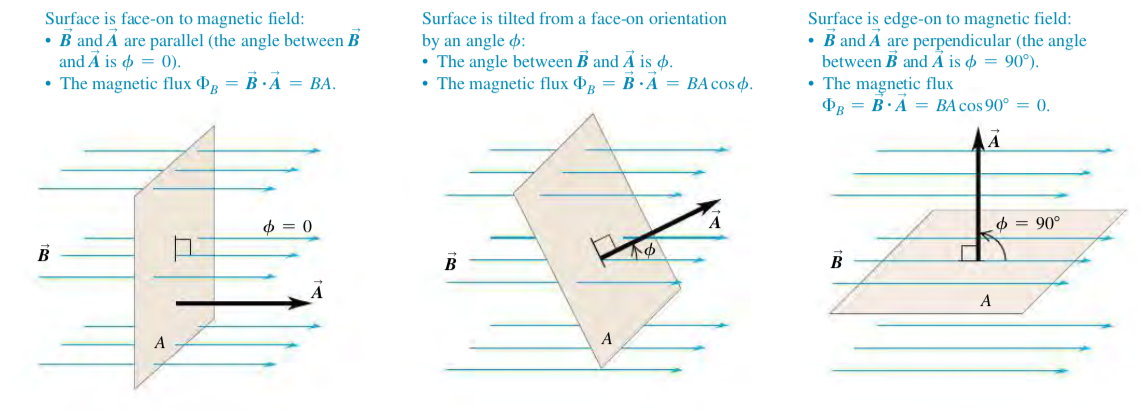
\includegraphics[scale=0.80]{images/faraday's_flux.png}

    \item If $\vec{\mathbf{B}}$ is uniform over $\vec{\mathbf{A}}$, then
        \begin{equation}
            \Phi_B = \vec{\mathbf{B}} \bigcdot \vec{\mathbf{A}} = BA\cos\phi
        \end{equation}
    \item \textbf{Faraday's Law of Induction} states:
        \begin{equation}
            \mathcal{E} = -\frac{d\Phi_B}{dt}
        \end{equation}
    \item Direction of induced emf can be calculated by finding the directions of
        $\vec{\mathbf{B}}$ and $\vec{\mathbf{A}}$, and determining the sign of magnitude
        flux $\Phi_B$ and its rate of change $\frac{d\Phi_B}{dt}$, then using the right
        hand rule:

        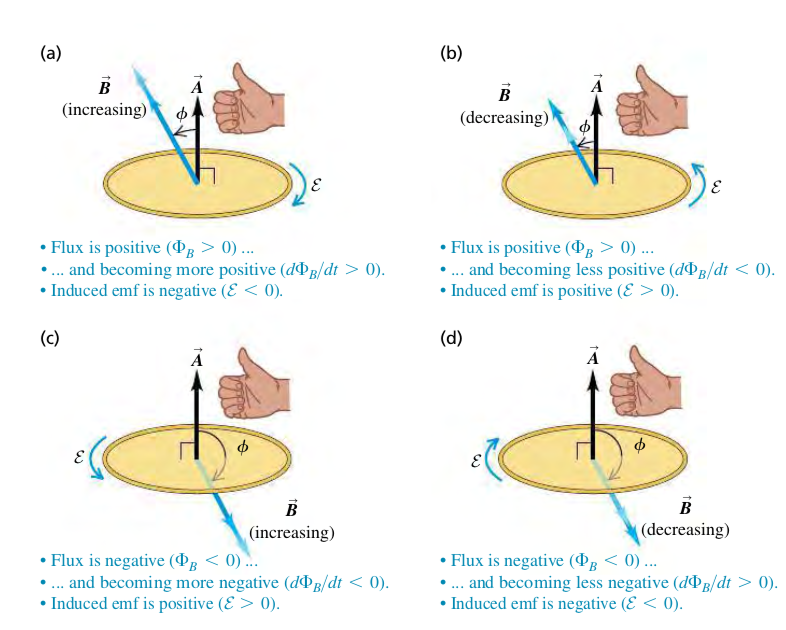
\includegraphics[scale=0.65]{images/faraday's_rhr.png}

    \item If a coil has $N$ identical turns and if the flux varies at the same rate
        through each turn, the total rate of change through all turns is:
        \begin{equation}
            \mathcal{E} = -N\frac{d\Phi_B}{dt}
        \end{equation}
\end{itemize}

\section[29.3, Lenz's Law]{Lenz's Law}
\begin{itemize}
    \item The direction of any magnetic induction effect is such as to oppose the cause
        of the effect

        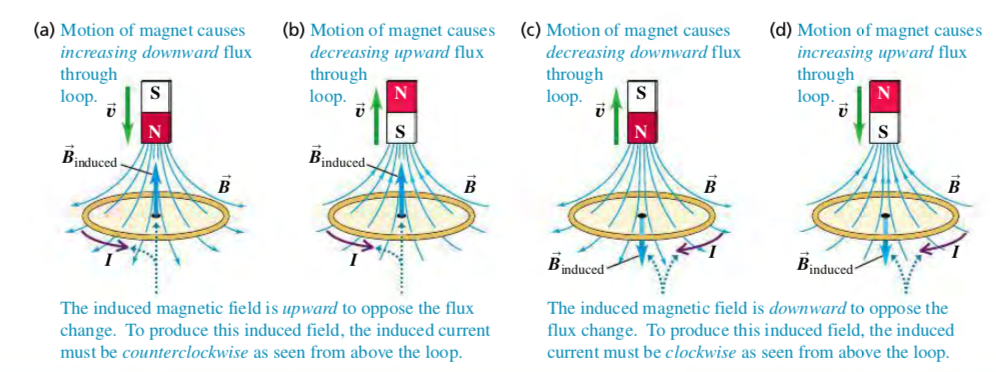
\includegraphics[scale=0.65]{images/induced_cur_dir.png}

    \item Lenz's Law gives only the direction of the induced current; the magnitude of
        the current depends only on the resistance of the circuit
    \item The less the circuit resistance, the greater the induced current and the more
        difficult it is to change flux
\end{itemize}


\section[29.4, Motional Electromotive Force]{Motional Electromotive Force}
\begin{itemize}
    \item The magnitude of the potential difference $V_{ab} = V_a - V_b$ is equal to the
        electric field magnitude $E$ multiplied by the length $L$ of the rod. Since
        $E=vB$, we have that:
        \begin{equation}
            V_{ab} = EL = vBL
        \end{equation}
    \item Emf is called a motional electromotive force, denoted by $\mathcal{E}$, which
        can be expressed as:
        \begin{equation}
            \mathcal{E} = vBL
        \end{equation}
    \item This can be generalized to any shape, for an element $d\vec{\mathbf{l}}$, of
        the conductor, the contribution $d\mathcal{E}$ to the emf is calculated as:
        \begin{equation}
            d\mathcal{E} = (\vec{\mathbf{v}} \times \vec{\mathbf{B}}) \bigcdot
            d\vec{\mathbf{l}}
        \end{equation}
    \item For any closed conducting loop, the total emf is:
        \begin{equation}
            \mathcal{E} = \oint (\vec{\mathbf{v}} \times \vec{\mathbf{B}})
            \bigcdot d\vec{\mathbf{l}}
        \end{equation}
    \item This expression is equivalent to Faraday's Law, but it must be used for
        conductors in motion
\end{itemize}

\section[29.5, Induced Electric Fields]{Induced Electric Fields}
\begin{itemize}
    \item A current I in the winding of the solenoid sets up a magnetic field
        $\vec{\mathbf{B}}$ along the solenoid axis. With $B=\mu_0 nI$, where $n$ is the
        number of turns per unit length
    \item If we take the area vector $\vec{\mathbf{A}}$ to point in the same direction as
        $\vec{\mathbf{B}}$, then the magnetic flux through the loop is
        \begin{equation}
            \Phi_B = BA = \mu_0 nIA
        \end{equation}
    \item When the solenoid current $I$ changes with time, the magnetic flux $\Phi_B$
        also changes, and the induced emf in the loop is:
        \begin{equation}
            \mathcal{E} = -\frac{d\vec{\mathbf{\Phi_B}}}{dt} =
            -\mu_0 nA\frac{dI}{dt}
        \end{equation}
    \item The total resistance of the loop is $R$, the induced current in the loop is
        \begin{equation}
            I^{\prime} = \frac{\mathcal{E}}{R}
        \end{equation}
    \item There must be an induced electric field in the conductor that is causeing the
        charges to move around the wire loop
    \item This electric field can be related to the emf as follows:
        \begin{equation}
            \oint \vec{\mathbf{E}} \bigcdot d\vec{\mathbf{l}} = \mathcal{E} =
            - \frac{d\vec{\mathbf{\Phi_B}}}{dt}
        \end{equation}
\end{itemize}

\section[29.6, Displacement Current and Maxwell's Equations]{Displacement Current and
    Maxwell's Equations}
\begin{itemize}
    \item Gauss's law for $\vec{\mathbf{E}}$:
        \begin{equation}
            \oint \vec{\mathbf{E}} \bigcdot d\vec{\mathbf{A}} =
            \frac{Q_{encl}}{\epsilon_0}
        \end{equation}
    \item The Second law involing $\vec{\mathbf{E}}$ and $\vec{\mathbf{B}}$ isthe
        analgous relationship for magnetic fields
        \begin{equation}
            \oint \vec{\mathbf{B}} \bigcdot d\vec{\mathbf{A}} = 0
        \end{equation}
    \item The third and fourth equations involve the line integral of $\vec{\mathbf{E}}$
        or $\vec{\mathbf{B}}$ around a closed path. Faraday's law states that a changing
        magnetic flux acts as a source of electriic field:
        \begin{equation}
            \oint \vec{\mathbf{B}} \bigcdot d\vec{\mathbf{l}} =
            - \frac{d\Phi_B}{dt}
        \end{equation}
    \item The fourth equation is Ampere's Law including displacement current:
        \begin{equation}
            \oint \vec{\mathbf{B}} \bigcdot d\vec{\mathbf{l}} =
            \mu_0\bigg(i_C + \epsilon_0 \frac{d\Phi_B}{dt}\bigg)
        \end{equation}
    \item Note that the electric field $\vec{\mathbf{E}}$ can be comprised of 2
        components, the electrostatic field $\vec{\mathbf{E_c}}$ and the nonelectrostatic
        field $\vec{\mathbf{E_n}}$, then:
        \begin{equation}
            \vec{\mathbf{E}} = \vec{\mathbf{E_c}} + \vec{\mathbf{E_n}}
        \end{equation}
\end{itemize}
\end{document}
